\section{Результаты}

\subsection{Эксперимент 1 --- базовый препроцессинг}

Результаты всех моделей на тестовой выборке приведены в таблице~\ref{tab:results_v1}.

\begin{table}[h]
\centering
\caption{Macro F1 и per-entity F1 на тесте (эксперимент 1)}
\label{tab:results_v1}
\small
\begin{tabular}{lrrrrrrr}
\toprule
\textbf{Модель} & \textbf{Macro} & \textbf{Gen.} & \textbf{Mat.} & \textbf{Met.} & \textbf{Metr.} & \textbf{OST} & \textbf{Task} \\
\midrule
bert\_linear\_noweight        & 0.604 & 0.714 & 0.557 & 0.681 & 0.573 & 0.531 & 0.565 \\
bert\_linear                  & 0.594 & 0.656 & 0.568 & 0.676 & 0.593 & 0.523 & 0.546 \\
roberta\_linear\_noweight     & 0.591 & 0.692 & 0.561 & 0.671 & 0.548 & 0.519 & 0.556 \\
roberta\_linear               & 0.585 & 0.673 & 0.557 & 0.651 & 0.593 & 0.531 & 0.505 \\
scibert\_linear\_noweight     & \textbf{0.646} & 0.712 & 0.659 & 0.749 & 0.618 & 0.566 & 0.571 \\
scibert\_linear               & 0.603 & 0.688 & 0.615 & 0.725 & 0.533 & 0.545 & 0.515 \\
scibert\_mlp                  & 0.644 & 0.708 & 0.665 & 0.746 & 0.615 & 0.577 & 0.553 \\
scibert\_linear\_crf\_noweight& 0.628 & 0.721 & 0.628 & 0.723 & 0.543 & 0.570 & 0.581 \\
scibert\_linear\_crf          & 0.628 & 0.721 & 0.628 & 0.723 & 0.543 & 0.570 & 0.581 \\
scibert\_concat4              & 0.644 & 0.737 & 0.661 & 0.751 & 0.573 & 0.579 & 0.561 \\
\bottomrule
\end{tabular}
\end{table}

\noindent{\small Gen.~= Generic, Mat.~= Material, Met.~= Method, Metr.~= Metric, OST~= OtherScientificTerm.}

\begin{figure}[h]
    \centering
    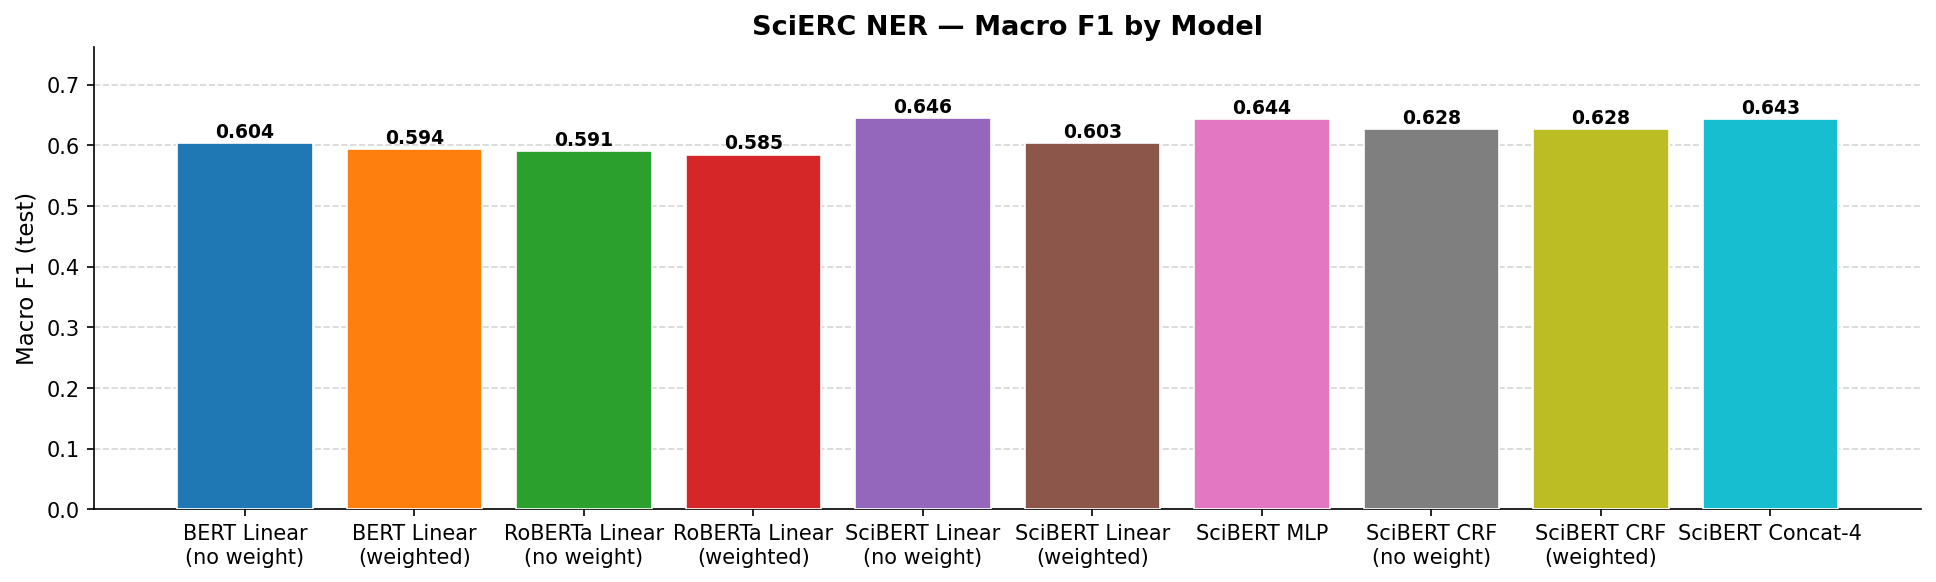
\includegraphics[width=\textwidth]{../plots/v1/macro_f1_comparison.png}
    \caption{Macro F1 по моделям (эксперимент 1)}
    \label{fig:macro_f1_v1}
\end{figure}

% ── 4.1.1 ──────────────────────────────────────────────────────────────────
\subsubsection{Влияние предобучения: SciBERT vs BERT vs RoBERTa}

Наиболее значимый фактор --- качество предобучения энкодера. \texttt{scibert\_linear\_noweight} (0.646) превосходит лучший BERT (\texttt{bert\_linear\_noweight}, 0.604) на 4.2~п.п. и лучший RoBERTa (\texttt{roberta\_linear\_noweight}, 0.591) на 5.5~п.п.

Разрыв максимален на типах Material и Method --- именно там, где доменная специфика проявляется сильнее всего. Material включает названия датасетов и ресурсов (\textit{Penn Treebank}, \textit{ImageNet}): SciBERT, обученный на научных статьях, видел эти упоминания многократно, тогда как BERT знает их лишь из Википедии. По Material SciBERT даёт 0.659 против 0.557 у BERT~--- разрыв 10~п.п.

RoBERTa несмотря на более агрессивное предобучение уступает BERT на большинстве типов. Возможная причина: RoBERTa обучена без NSP (Next Sentence Prediction), что снижает её чувствительность к межпредложенческим зависимостям. Кроме того, BPE-токенизация RoBERTa хуже справляется с редкими научными терминами по сравнению с WordPiece BERT.

% ── 4.1.2 ──────────────────────────────────────────────────────────────────
\subsubsection{Взвешивание классов: noweight стабильно лучше}

Во всех парах вариант без взвешивания превосходит взвешенный: разрыв составляет от 0.6~п.п. (RoBERTa) до 4.3~п.п. (SciBERT). Это противоречит интуиции, но объясняется механизмом ошибок.

Взвешивание усиливает штраф за пропуск редких классов (Metric, Task), но одновременно снижает штраф за пропуск частых (Generic, Method, \texttt{O}). На уровне отдельных типов видно: \texttt{scibert\_linear} (взвешенный) имеет Generic 0.688 против 0.712 у \texttt{scibert\_linear\_noweight} и Method 0.725 против 0.749. Модель начинает «видеть» сущности там, где их нет, --- растёт число ложных срабатываний на частых типах, что снижает их precision.

Выигрыш взвешивания на редких типах (Metric: +0.086 для BERT, +0.061 для RoBERTa) не компенсирует потерю на частых в рамках macro F1. Вывод: на данном датасете класс \texttt{O} настолько доминирует, что даже sqrt-сглаженное взвешивание сдвигает модель в сторону гиперчувствительности.

% ── 4.1.3 ──────────────────────────────────────────────────────────────────
\subsubsection{Архитектура головы: простое работает лучше}

Среди SciBERT-моделей без взвешивания результаты следующие:

\begin{center}
\begin{tabular}{lr}
\toprule
Голова & Macro F1 \\
\midrule
Linear      & \textbf{0.646} \\
MLP         & 0.644 \\
Concat-4    & 0.644 \\
Linear+CRF  & 0.628 \\
\bottomrule
\end{tabular}
\end{center}

\textbf{MLP и Concat-4} практически равны Linear ($\Delta < 0.002$). SciBERT-энкодер настолько мощный, что добавление нелинейности или многоуровневых признаков не даёт значимого прироста. При этом MLP и Concat-4 сложнее в обучении: у MLP больше параметров, у Concat-4 --- нестандартный forward-pass, что потенциально увеличивает дисперсию.

\textbf{CRF} показывает худший результат среди SciBERT-моделей: 0.628, на 1.8~п.п. ниже линейной головы. Причин несколько. Во-первых, BERT-энкодер уже неявно моделирует зависимости между метками: контекстуализированные представления содержат информацию о соседних токенах, и BIO-согласованность возникает как следствие, а не должна задаваться явно. Во-вторых, CRF-loss оптимизирует правдоподобие всей последовательности целиком, что делает обучение менее стабильным на малом датасете. В-третьих, применение весов классов через умножение эмиссий (вместо корректного включения в маргинальное распределение CRF) является приближением.

% ── 4.1.4 ──────────────────────────────────────────────────────────────────
\subsubsection{Анализ по типам сущностей}

\begin{figure}[h]
    \centering
    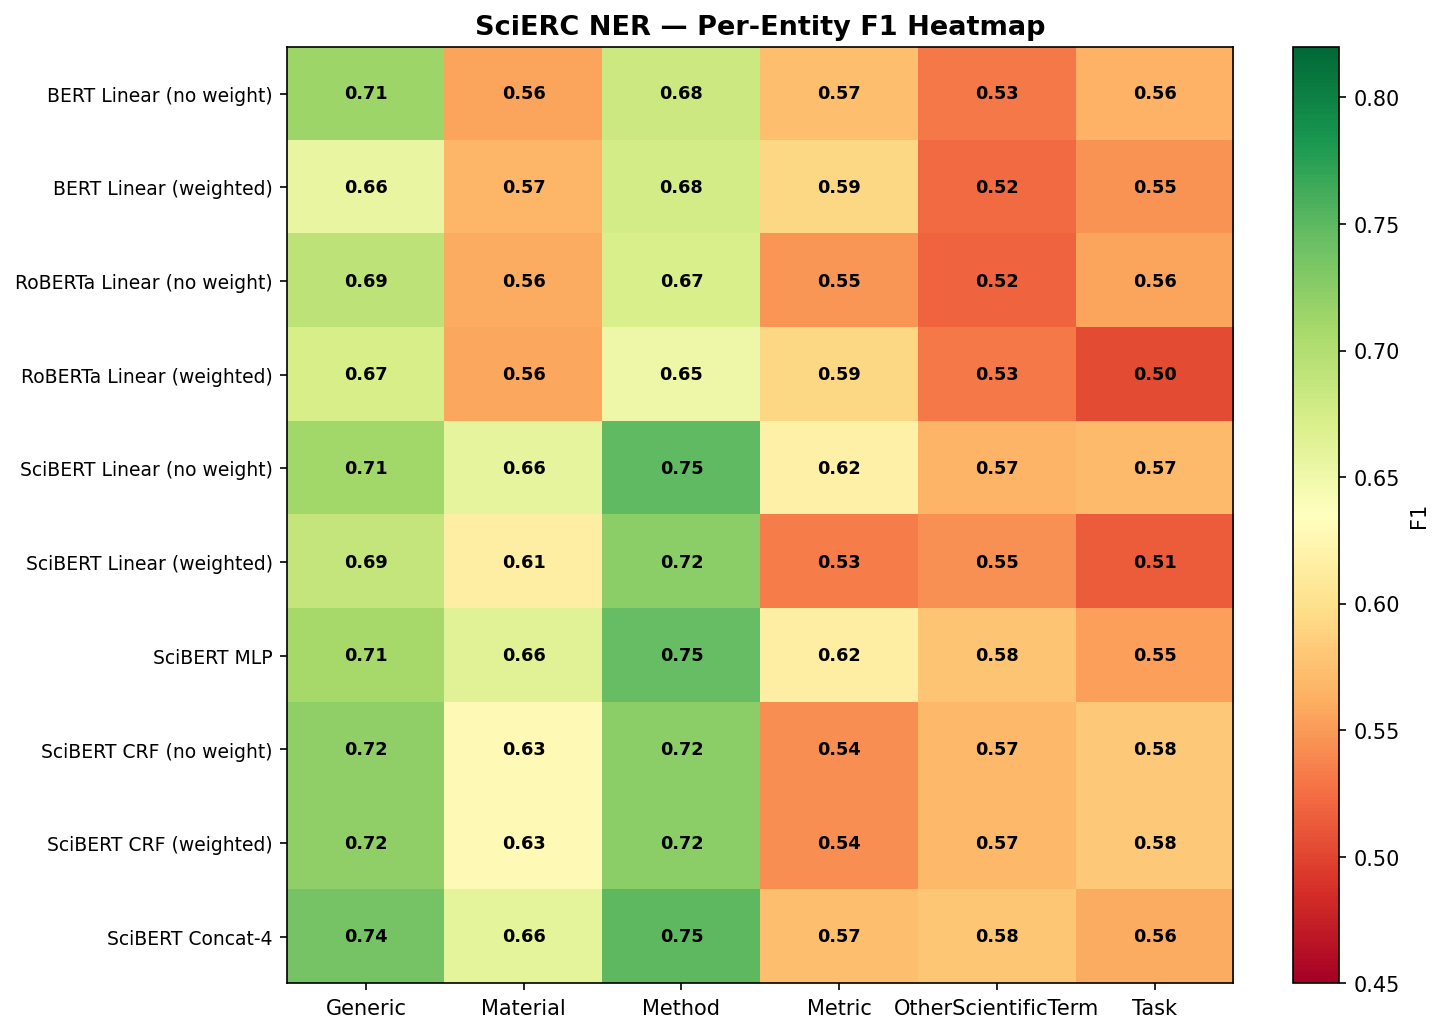
\includegraphics[width=\textwidth]{../plots/v1/entity_f1_heatmap.png}
    \caption{Тепловая карта per-entity F1 (эксперимент 1)}
    \label{fig:heatmap_v1}
\end{figure}

Рисунок~\ref{fig:heatmap_v1} позволяет выявить следующие закономерности.

\textbf{Method} --- лучше всего распознаётся всеми моделями (0.65--0.75). Названия методов имеют отчётливые контекстные сигналы: «\textit{we propose}», «\textit{based on}», «\textit{model}».

\textbf{Generic} --- высокий F1 (0.66--0.74), хотя это «мусорная корзина» для трудно категоризируемых терминов. Объяснение: Generic-сущности частотны, модель видит достаточно примеров.

\textbf{Material} --- высокая дисперсия (0.56--0.66). Наиболее чувствителен к доменному предобучению: именно здесь SciBERT отрывается от BERT/RoBERTa.

\textbf{Metric} --- стабильно трудный тип (0.53--0.62). Многие метрики --- короткие аббревиатуры (\textit{F1}, \textit{BLEU}, \textit{ROUGE}), которые встречаются в разных контекстах и легко путаются с Generic или Method.

\textbf{OtherScientificTerm} --- самый низкий F1 (0.52--0.58) по всем моделям. Это ожидаемо: OST --- остаточная категория без чёткого семантического ядра, куда попадают все термины, не вошедшие в другие типы.

\textbf{Task} --- 0.50--0.58, близко к OST. Описания задач разнообразны и часто многословны (\textit{machine translation}, \textit{named entity recognition}), что усложняет определение точных границ span'а.

% ── 4.1.5 ──────────────────────────────────────────────────────────────────
\subsubsection{Анализ матриц ошибок}

\begin{figure}[h]
    \centering
    \begin{subfigure}[b]{0.48\textwidth}
        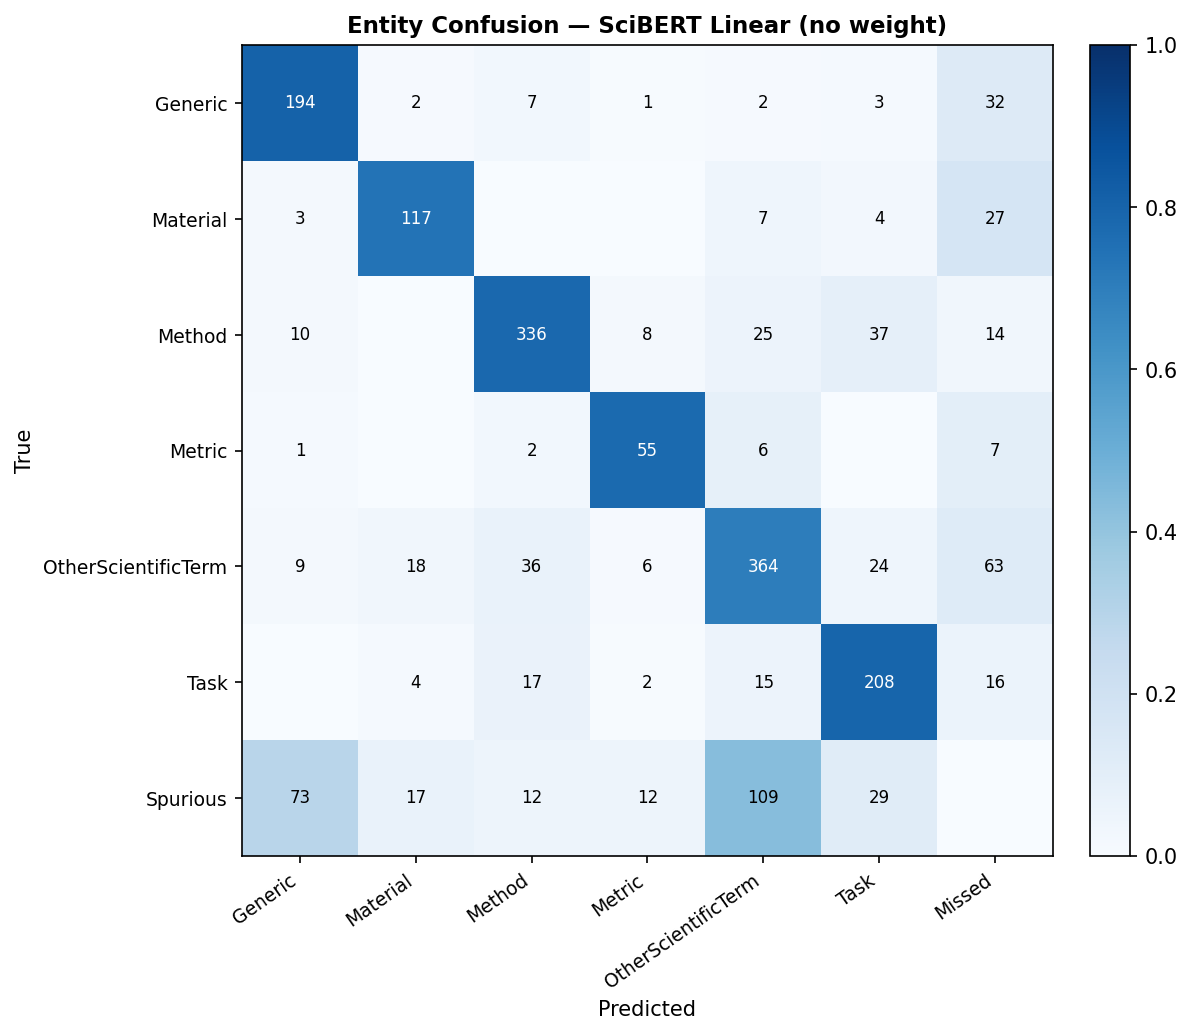
\includegraphics[width=\textwidth]{../plots/v1/conf_mtx/scibert_linear_noweight.png}
        \caption{scibert\_linear\_noweight (лучшая модель)}
    \end{subfigure}
    \hfill
    \begin{subfigure}[b]{0.48\textwidth}
        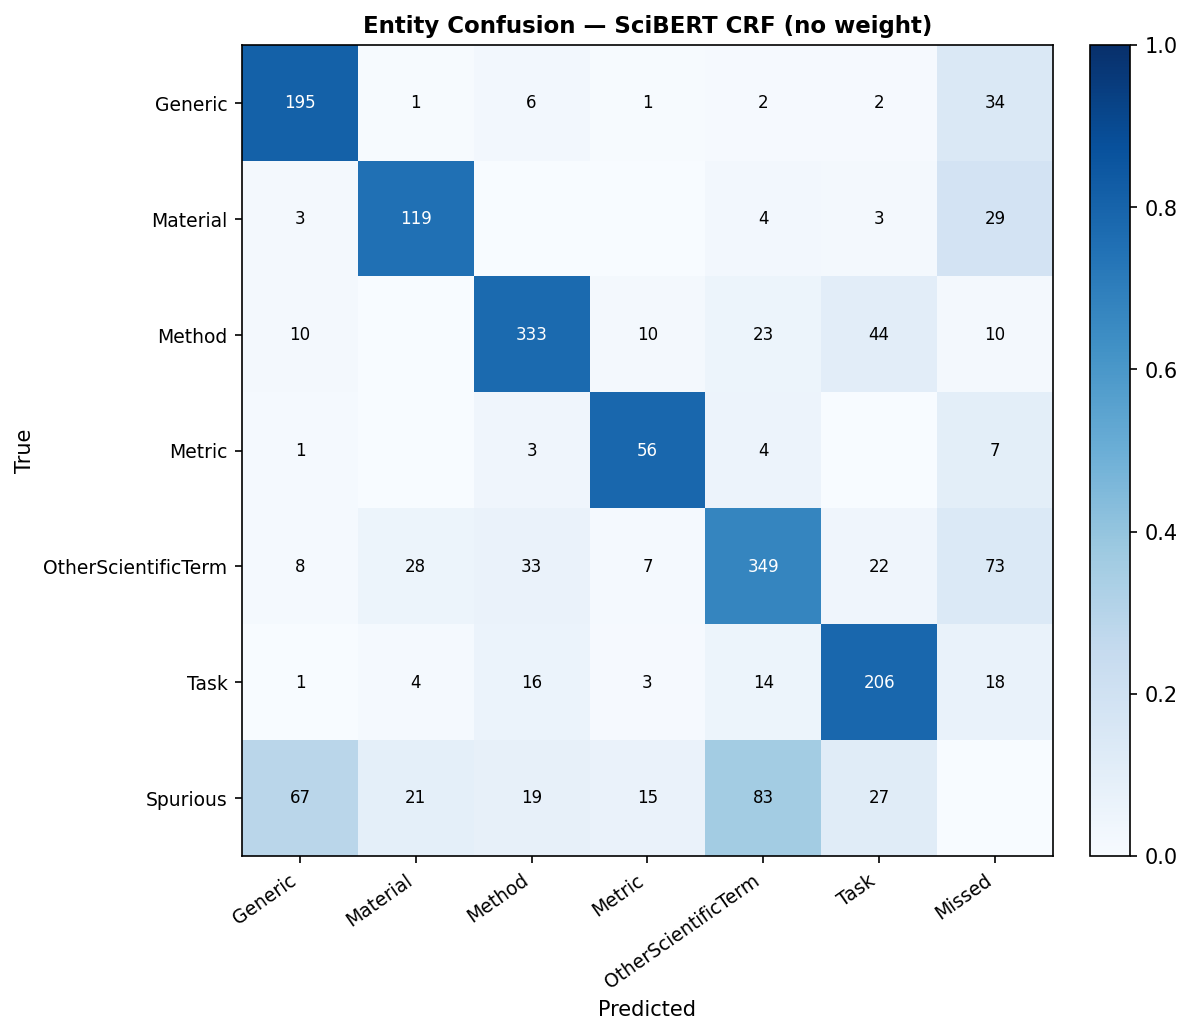
\includegraphics[width=\textwidth]{../plots/v1/conf_mtx/scibert_linear_crf_noweight.png}
        \caption{scibert\_linear\_crf\_noweight}
    \end{subfigure}
    \caption{Матрицы ошибок (нормировано по строкам; «Missed»~= FN, «Spurious»~= FP)}
    \label{fig:conf_mtx_v1}
\end{figure}

Матрицы строятся на уровне сущностей: строка соответствует истинному типу, столбец --- предсказанному. Ячейка «Missed» --- пропущенные сущности (FN), строка «Spurious» --- ложные срабатывания (FP).

Matching между истинными и предсказанными спанами выполняется по перекрытию: истинный спан сопоставляется с предсказанным, если они делят хотя бы одну позицию токена. Это позволяет отделить ошибки типа (правильные границы, неверный класс) от пропусков (спан не найден вообще).

Ключевые наблюдения:

\textbf{Пропуски доминируют, но межтиповая путаница значима.} Для большинства типов столбец «Missed» наибольший, однако после перехода на overlap-matching видна реальная путаница: Method $\to$ OtherScientificTerm (25 случаев), Task $\to$ Method (17), OtherScientificTerm $\to$ Material (18). Эти ошибки семантически объяснимы: границы между смежными категориями размыты.

\textbf{Generic и OtherScientificTerm --- главные источники путаницы.} Оба типа --- «мусорные корзины» для трудно категоризируемых понятий, поэтому модель систематически их смешивает. Это структурная проблема разметки, а не слабость модели.

\textbf{Редкие типы пропускаются чаще.} Metric и Task имеют наибольшую долю в столбце «Missed» относительно общего числа истинных сущностей --- что согласуется с их низким F1 и малым числом примеров в обучающей выборке.

\textbf{CRF не снижает число пропусков.} Матрица ошибок CRF-модели похожа на линейную голову: CRF улучшает BIO-согласованность токенов, но не помогает модели находить трудные спаны.

% ── 4.1.6 ──────────────────────────────────────────────────────────────────
\subsubsection{Кривые обучения}

\begin{figure}[h]
    \centering
    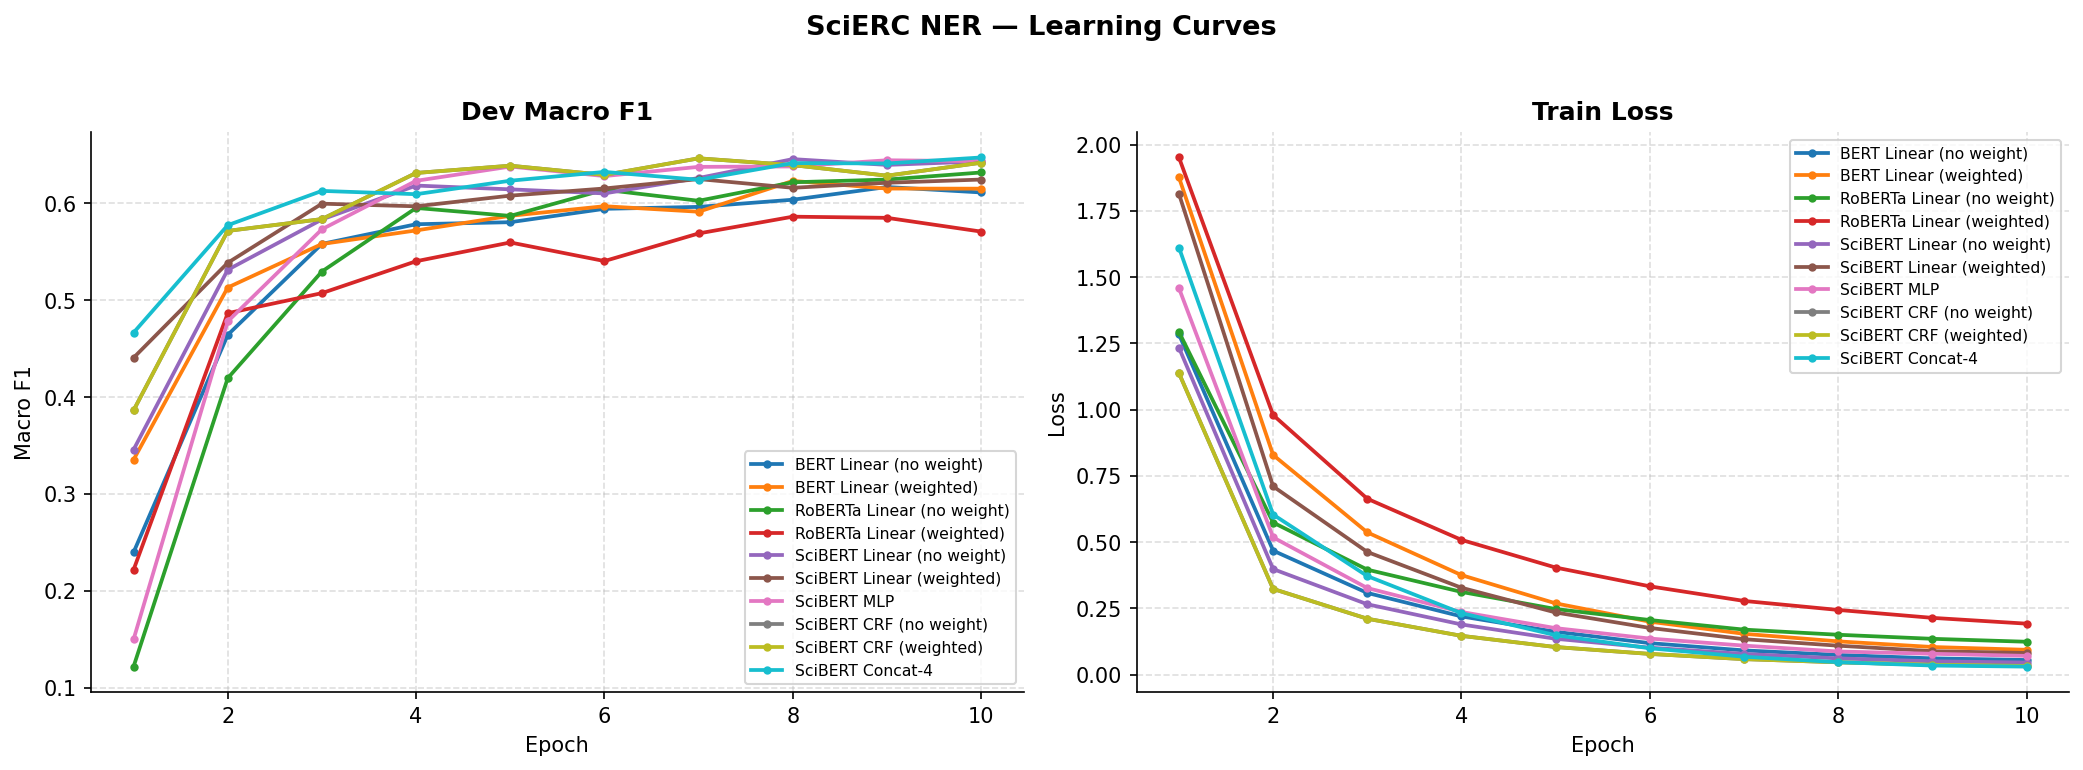
\includegraphics[width=\textwidth]{../plots/v1/learning_curves.png}
    \caption{Dev macro F1 и train loss по эпохам (эксперимент 1)}
    \label{fig:curves_v1}
\end{figure}

SciBERT-модели выходят на плато к эпохе 7--8, BERT~--- к 8--10. Это соответствует более высокому starting point SciBERT: он ближе к целевому распределению уже после первой эпохи файн-тюнинга. RoBERTa демонстрирует заметную нестабильность на первых 3--4 эпохах: большой learning rate (тот же $2 \times 10^{-5}$, что и для остальных) может быть завышен для её архитектуры при таком малом датасете.

CRF-модели имеют более высокий начальный train loss и медленнее убывают~--- CRF оптимизирует правдоподобие последовательности, что труднее, чем токен-уровневая кросс-энтропия.

% ── 4.1.7 ──────────────────────────────────────────────────────────────────
\subsubsection{Сравнение с опубликованными результатами}

На SciERC лучшие опубликованные результаты для задачи только NER достигаются span-based моделями: DyGIE++~\cite{wadden2019dygiepp} сообщает F1~$\approx 0.67$--$0.68$. Наш лучший результат (0.646) уступает примерно на 2--3~п.п.

Разрыв объясним методологически: span-based подходы напрямую классифицируют кандидатные span'ы, избегая ошибок выравнивания субтокенов, и часто обучаются совместно с задачей извлечения отношений (multi-task learning), что даёт дополнительный обучающий сигнал. Token-level BIO является упрощением, при котором ошибка в одном токене разрушает весь span.

% ── 4.2 ────────────────────────────────────────────────────────────────────
\subsection{Эксперимент 2 --- улучшенный препроцессинг}

Результаты всех моделей с добавлением entity swap аугментации и контекстного окна (window~$= 1$) приведены в таблице~\ref{tab:results_v2}.

\begin{table}[h]
\centering
\caption{Macro F1 и per-entity F1 на тесте (эксперимент 2)}
\label{tab:results_v2}
\small
\begin{tabular}{lrrrrrrr}
\toprule
\textbf{Модель} & \textbf{Macro} & \textbf{Gen.} & \textbf{Mat.} & \textbf{Met.} & \textbf{Metr.} & \textbf{OST} & \textbf{Task} \\
\midrule
bert\_linear\_noweight        & 0.575 & 0.685 & 0.540 & 0.679 & 0.533 & 0.496 & 0.521 \\
bert\_linear                  & 0.605 & 0.673 & 0.565 & 0.683 & 0.613 & 0.537 & 0.557 \\
roberta\_linear\_noweight     & 0.594 & 0.641 & 0.598 & 0.688 & 0.588 & 0.522 & 0.528 \\
roberta\_linear               & 0.598 & 0.674 & 0.607 & 0.661 & 0.584 & 0.524 & 0.537 \\
scibert\_linear\_noweight     & \textbf{0.654} & 0.727 & 0.632 & 0.757 & 0.630 & 0.592 & 0.584 \\
scibert\_linear               & 0.642 & 0.723 & 0.628 & 0.736 & 0.641 & 0.573 & 0.552 \\
scibert\_mlp                  & 0.648 & 0.723 & 0.632 & 0.740 & 0.667 & 0.567 & 0.558 \\
scibert\_linear\_crf\_noweight& 0.650 & 0.727 & 0.645 & 0.738 & 0.587 & 0.598 & 0.605 \\
scibert\_linear\_crf          & 0.459 & 0.275 & 0.433 & 0.654 & 0.299 & 0.542 & 0.550 \\
scibert\_concat4              & 0.618 & 0.722 & 0.632 & 0.704 & 0.564 & 0.553 & 0.535 \\
\bottomrule
\end{tabular}
\end{table}

\noindent{\small Gen.~= Generic, Mat.~= Material, Met.~= Method, Metr.~= Metric, OST~= OtherScientificTerm.}

\begin{figure}[h]
    \centering
    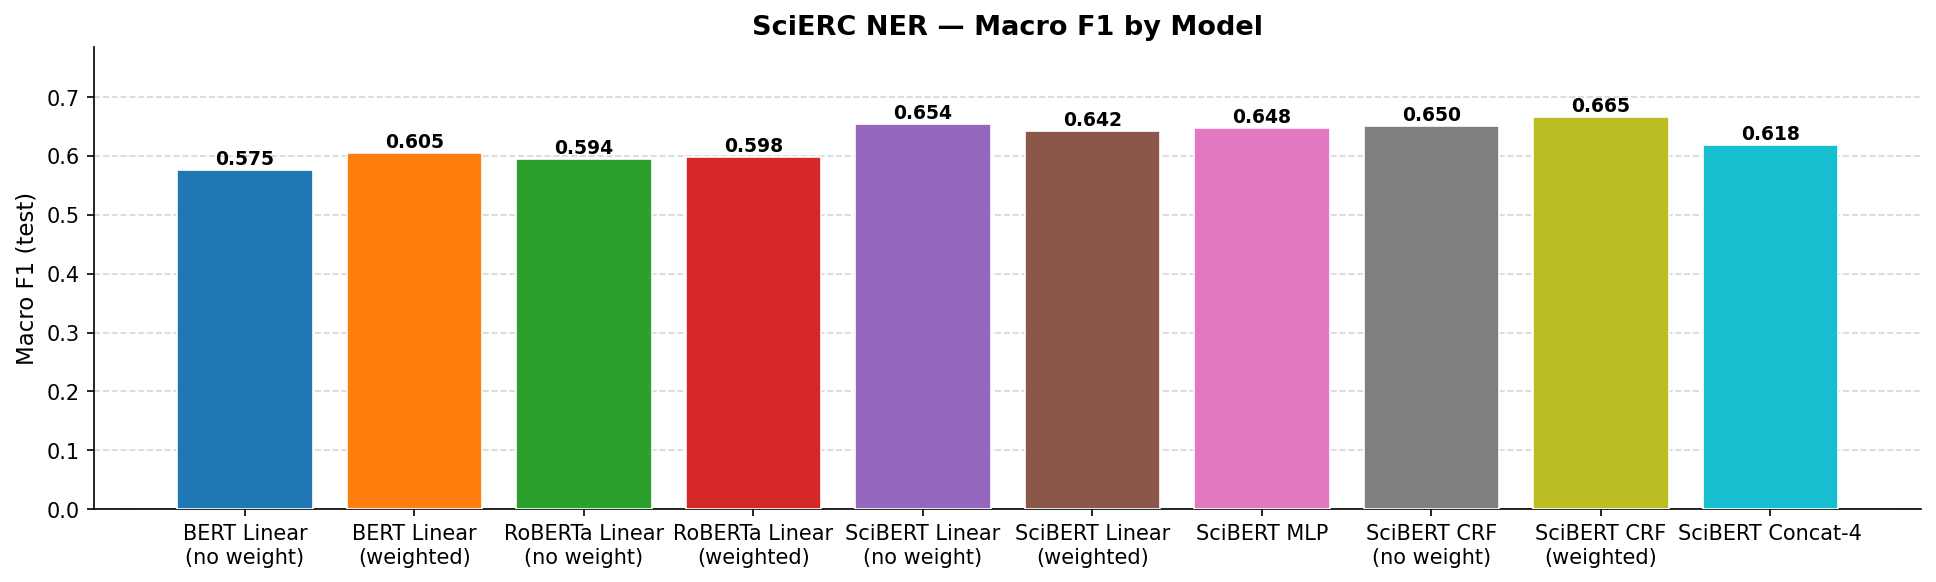
\includegraphics[width=\textwidth]{../plots/v2/macro_f1_comparison.png}
    \caption{Macro F1 по моделям (эксперимент 2)}
    \label{fig:macro_f1_v2}
\end{figure}

% ── 4.2.1 ──────────────────────────────────────────────────────────────────
\subsubsection{Общая картина: кто выиграл, кто проиграл}

Из 10 моделей 7 улучшились или остались на прежнем уровне; 3 показали деградацию.
Сводное сравнение $\Delta$~macro~F1 между экспериментами 1 и 2:

\begin{center}
\begin{tabular}{lrrr}
\toprule
Модель & Exp.~1 & Exp.~2 & $\Delta$ \\
\midrule
scibert\_linear        & 0.603 & \textbf{0.642} & $+$3.9~п.п. \\
scibert\_linear\_crf\_noweight & 0.628 & 0.650 & $+$2.2~п.п. \\
roberta\_linear        & 0.585 & 0.598 & $+$1.3~п.п. \\
bert\_linear           & 0.594 & 0.605 & $+$1.1~п.п. \\
scibert\_linear\_noweight & 0.646 & 0.654 & $+$0.8~п.п. \\
scibert\_mlp           & 0.644 & 0.648 & $+$0.4~п.п. \\
roberta\_linear\_noweight & 0.591 & 0.594 & $+$0.3~п.п. \\
\midrule
scibert\_concat4       & 0.644 & 0.618 & $-$2.5~п.п. \\
bert\_linear\_noweight & 0.604 & 0.575 & $-$2.8~п.п. \\
scibert\_linear\_crf   & 0.628 & 0.459 & $-$16.9~п.п. \\
\bottomrule
\end{tabular}
\end{center}

% ── 4.2.2 ──────────────────────────────────────────────────────────────────
\subsubsection{Аугментация сокращает разрыв между взвешенной и невзвешенной моделью}

Самый значимый результат эксперимента~2 --- драматичный рост \texttt{scibert\_linear} ($+3.9$~п.п.), который стал лучшей взвешенной моделью. В эксперименте~1 разрыв между \texttt{scibert\_linear\_noweight} и \texttt{scibert\_linear} составлял $4.3$~п.п. В эксперименте~2 он сократился до $1.2$~п.п.

Механизм объясняется через Metric F1: в эксперименте~1 \texttt{scibert\_linear} давал~$0.532$, в эксперименте~2 ---~$0.641$ ($+10.9$~п.п.). Entity swap аугментация создаёт новые предложения, в которых редкие сущности (Metric, Task) появляются в новых контекстах: модель видит больше примеров этих типов, и необходимость искусственно усиливать их вес через $w_c$ снижается. В то же время взвешивание по-прежнему предотвращает коллапс модели на класс \texttt{O}, что даёт небольшой прирост относительно \texttt{scibert\_linear\_noweight}.

% ── 4.2.3 ──────────────────────────────────────────────────────────────────
\subsubsection{Аугментация без взвешивания приводит к деградации}

\texttt{bert\_linear\_noweight} потерял $2.8$~п.п. и показал спад по всем типам сущностей.
В эксперименте~1 эта модель была лучшей среди BERT-моделей (0.604); в эксперименте~2 она стала худшей из BERT.

Без взвешивания классов аугментированные предложения с рандомно переставленными сущностями создают шум: модель видит одни и те же токены с разными метками в зависимости от того, в какой контекст они попали при свапе. Взвешивание смягчает этот эффект, концентрируя сигнал на редких классах; у \texttt{bert\_linear} (с весами) результат вырос на $1.1$~п.п.

% ── 4.2.4 ──────────────────────────────────────────────────────────────────
\subsubsection{CRF с весами классов сломан}

\texttt{scibert\_linear\_crf} деградировал с~$0.628$ до~$0.459$ ($-16.9$~п.п.) и не может рассматриваться как рабочий результат. Generic F1 упал до~$0.275$ --- признак систематической путаницы классов.

В нашей реализации веса классов применяются как мультипликаторы эмиссионных потенциалов CRF, что является приближением. При базовом препроцессинге (эксперимент~1) это приближение давало приемлемые результаты, поскольку распределение токенов в батче было однородным. Контекстное окно (эксперимент~2) добавляет токены с меткой $-100$ (токены соседних предложений), которые не участвуют в CRF-лоссе, но изменяют статистику батча. Взаимодействие этого сдвига с мультипликативными весами дестабилизировало обучение. \texttt{scibert\_linear\_crf\_noweight} (без весов) при тех же условиях улучшился на $2.2$~п.п., что подтверждает: причина именно в совместном применении весов и CRF, а не в контекстном окне как таковом.

% ── 4.2.5 ──────────────────────────────────────────────────────────────────
\subsubsection{Влияние на типы сущностей}

\begin{figure}[h]
    \centering
    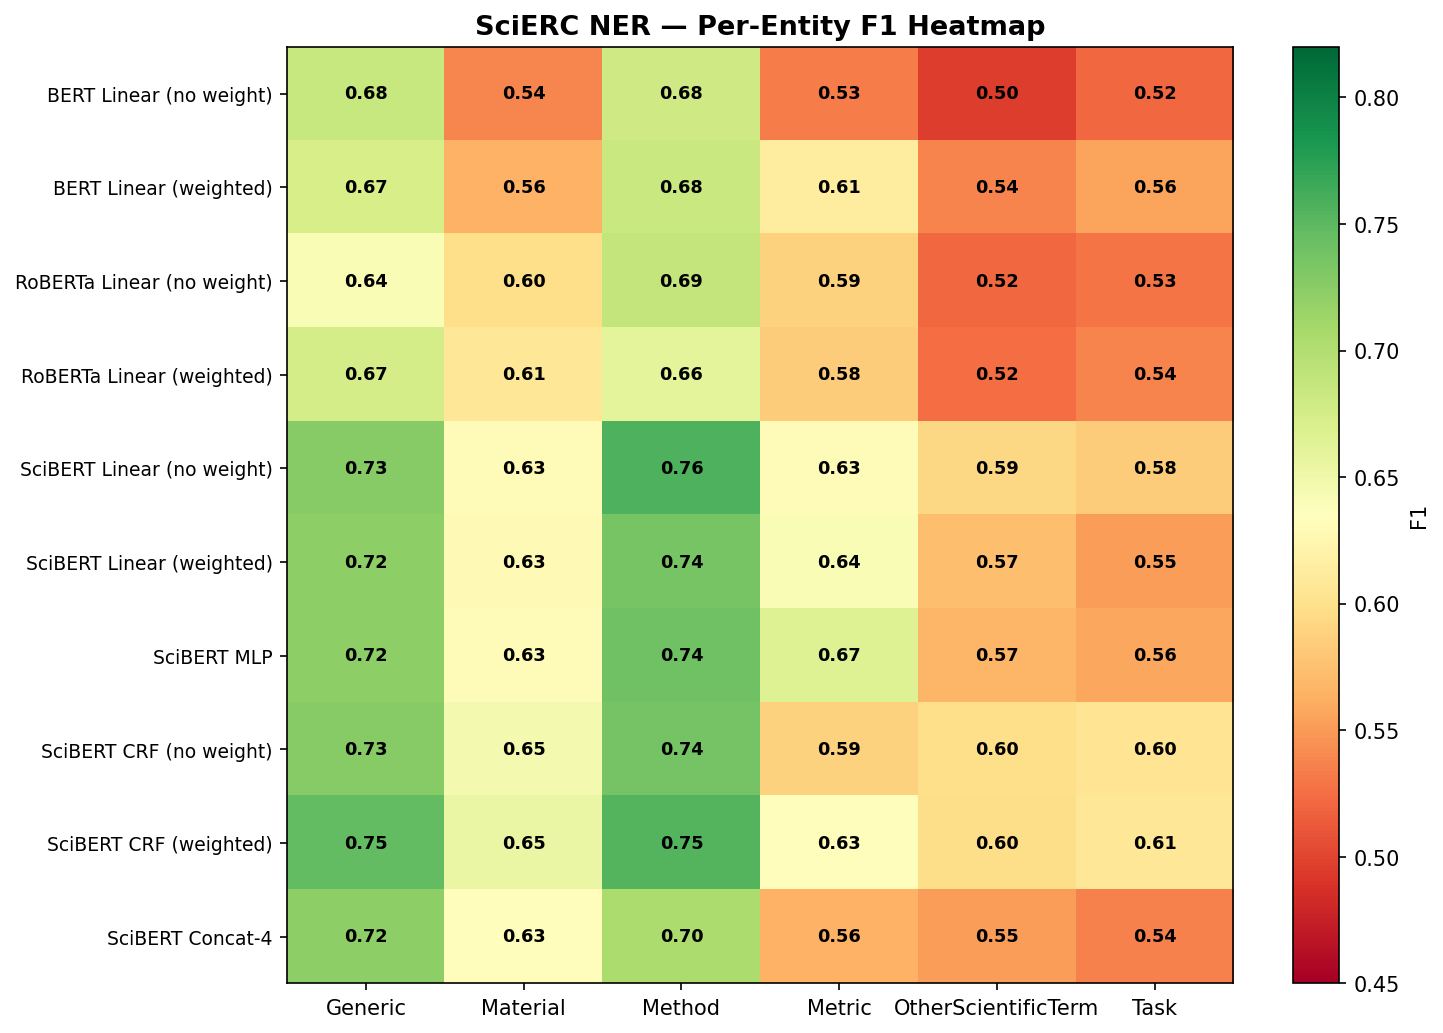
\includegraphics[width=\textwidth]{../plots/v2/entity_f1_heatmap.png}
    \caption{Тепловая карта per-entity F1 (эксперимент 2)}
    \label{fig:heatmap_v2}
\end{figure}

Наибольший прирост от улучшенного препроцессинга получают типы \textbf{Metric} и \textbf{Task} --- именно те, которые в эксперименте~1 распознавались хуже всего. По Metric лучшие SciBERT-модели вырастают с~$0.53$--$0.62$ до~$0.59$--$0.67$; по Task --- с~$0.51$--$0.58$ до~$0.55$--$0.61$. Это согласуется с механизмом entity swap: он создаёт дополнительный обучающий сигнал именно для редких типов.

Тип \textbf{Material} у SciBERT-моделей незначительно снизился ($-0.02$--$0.03$~п.п.). Возможное объяснение: свапы, при которых название датасета или ресурса вставлялось в предложение о другом материале, создавали синтетические примеры с нарушенной семантической связностью, что мешало модели обнаруживать Material в реальных текстах.

% ── 4.2.6 ──────────────────────────────────────────────────────────────────
\subsubsection{Лучшая модель и итоговый вывод}

Лучшим результатом эксперимента~2 остаётся \texttt{scibert\_linear\_noweight}~($0.654$) --- на $0.8$~п.п. выше, чем в эксперименте~1. Несмотря на то, что аугментация и контекстное окно дают статистически значимый прирост для большинства моделей, абсолютный выигрыш скромен.

Главный вывод: улучшенный препроцессинг не меняет иерархию моделей (SciBERT $\succ$ BERT $\approx$ RoBERTa), но сужает разрыв между взвешенными и невзвешенными вариантами и особенно помогает моделям, которые в эксперименте~1 страдали от редких типов. Он также обнажил проблему CRF с весами: этот вариант следует переработать с явным включением весов в маргинальное распределение вместо мультипликативного приближения.
